% !TEX root = ../../report.tex

\section{State Of The Art}
\label{sec:SotA}

This section will present and discuss previous work in the field of recommender systems, existing solutions to the cold-start problem and fashion recommender systems. The section will also contain a discussion of the domain specific challenges of designing a recommender system for the fashion domain.

\subsection{Recommender Systems foundations}

%TODO - Find a way to incorporate this in the introduction
%TODO - Write something about personalized recommendations (Amazon CEO quote, 8 million customers, 8 million stores)

%Personalized recommendations, what assumptions can be made?
%\#1 - You are like your friends
%\#2 - You are like people who do similar things that you do
%\#3 - You like things that are similar to things you already like
%\#4 - You are influenced by experts and the opinions of others

Recommender systems have become an important research topic since the introduction of Tapestry \cite{Goldberg1992}, the first collaborative filtering system back in 1992. Recommender systems now play an important role in many of the most popular web-sites such as Amazon, YouTube, Netflix, Tripadvisor, Last.fm, and IMDb. In its most common formulation the recommendation problem is reduced to the problem of estimating the preference/rating of items that have not been seen by a user. Usually, this estimation is based on ratings previously given by the user to other items in the collection. Once we have estimated these ratings we can recommend the items with the highest rating to the user. These recommendations relate to various decision-making processes, such as what items to buy, what music to listen to, or what online news to read. Recommender systems are usually classified into the following categories, based on how the recommendations are made \cite{Adomavicius2005}.

\begin{itemize}
\item \emph{Content-based recommendations:} The user will be recommended items with similar content to the ones the user preferred in the past;
\item \emph{Collaborative recommendations:} The user will be recommended items that people with similar testes and preferences have liked in the past;
\item \emph{Hybrid approaches:} These methods combine collaborative and content-based methods.
\end{itemize}

\subsubsection{Content Based Filtering}

In a content-based system, we must construct a \emph{profile} $ContentBasedProfile(c)$ or each user $c$, which is a record or collection of the attributes which characterizes each item $Content(s)$ of all the items $s_{i} \epsilon S$ previously rated by user $c$. For example in a fashion recommender system the content-based recommender system tries to understand the commonalities among the items user $c$ has rated highly in the past (color, brand, store, price, etc.). Then recommend items that have a high degree of similarity to these items. $ContentBasedProfile(c)$ can be designed as a vector of weights $(w_{c1} ... w_{ck})$, where each weight $w_{ci}$ denotes the importance of the keyword $k_{i}$ to user $c$.

Items that can be recommended to the user can often be stored in a database table. Figure \ref{figure:contentbaseddb} shows a simple database with rows describing 5 items that have been rated by 3 users. The column names starting with $X_{n}$ are the properties of the items, often referred to as "attributes".

\begin{figure}[H]
    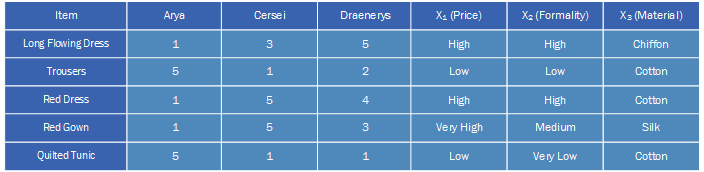
\includegraphics[width=5in]{image/contentbaseddb.png}
    \centering
    \caption[A clothing database]{A clothing database. Rows are items, columns are users and properties of the items}
    \label{figure:contentbaseddb}
\end{figure}

From the rating matrix and content properties one can then construct a $ContentBasedProfile(c)$ for each user $c$, for the user Arya one could imagine it would look something like this.

\begin{figure}[H]
    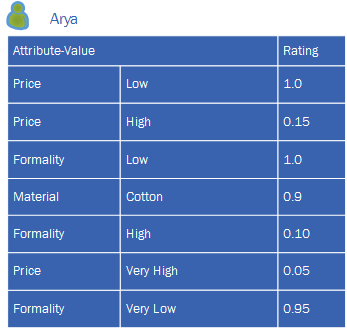
\includegraphics[width=2in]{image/contentprofile.png}
    \centering
    \caption[Content Profile Example]{Content Profile Example}
    \label{figure:contentprofile}
\end{figure}

The recommendation process consists of matching up the attributes of the user profile against the attributes of an item. The result is a relevance judgment that represents the user's level of interest in that object. The utility $u(c, s)$ of item $s$ for user $c$ is estimated based on the utilities $u(c, s_{i})$ assigned by user c to items $s_{i} \epsilon S$ that exhibit a similarity to item $s$. E.g. for the user Arya items with the attributes low price and low formality could safely be recommended as they fit her user profile, and have similar characteristics to the items which she previously have rated highly. The utility function $r(u, i)$ is usually defined as:
\begin{equation}
r(u,i) = score(ContentBasedProfile(u), Content(i)).
\end{equation}

\subsubsection{Collaborative Filtering}
\label{subsec:cf}

The goal of collaborative filtering methods is to suggest new items or to predict the utility $u(c, s)$ of a certain item s for a particular user c based on the user's previous activities and/or likings and similarity to other users. In a typical CF scenario, there is a list of $n$ users $C = {c_{1}, ... c_{n}}$ and a list of $m$ items $S = {s_{1},...s_{m}}$. Each user $c_{i}$ has a list of items $S_{si}$, which the user have expressed her opinion about, which makes up our rating matrix of size $S \times C$. More formally, the utility $u(c, s)$ of item $s$ for user $c$ is estimated based on the utilities $u(c_{j}, s)$ assigned to item $s$ by the users $c_{j} \epsilon C$, which can be considered "similar" to the active user $c$. This is exemplified in Figure \ref{figure:ratingmatrix}. For example, in our fashion recommender system, in order to recommend clothes to user $c$, the collaborative filtering method must find the "peers" of users $c$, which share the same tastes in clothes (user which tend to enjoy similar clothes). Then, recommend the clothes that are most liked among these "peers".

\begin{figure}[H]
    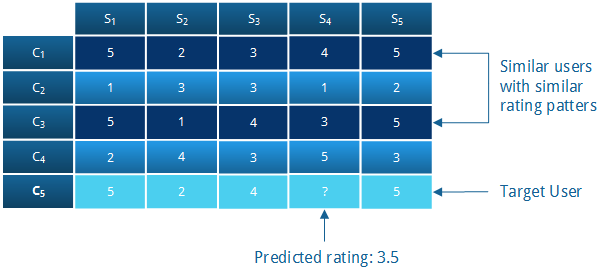
\includegraphics[width=5in]{image/ratingmatrix.png}
    \centering
    \caption[Collaborative filtering rating matrix]{Collaborative filtering rating matrix}
    \label{figure:ratingmatrix}
\end{figure}

Researchers have devised a number of collaborative filtering algorithms that can be divided into two main categories: Memory-based and Model-based algorithms \cite{Su2009}.\linebreak[4]

\begin{figure}[H]
    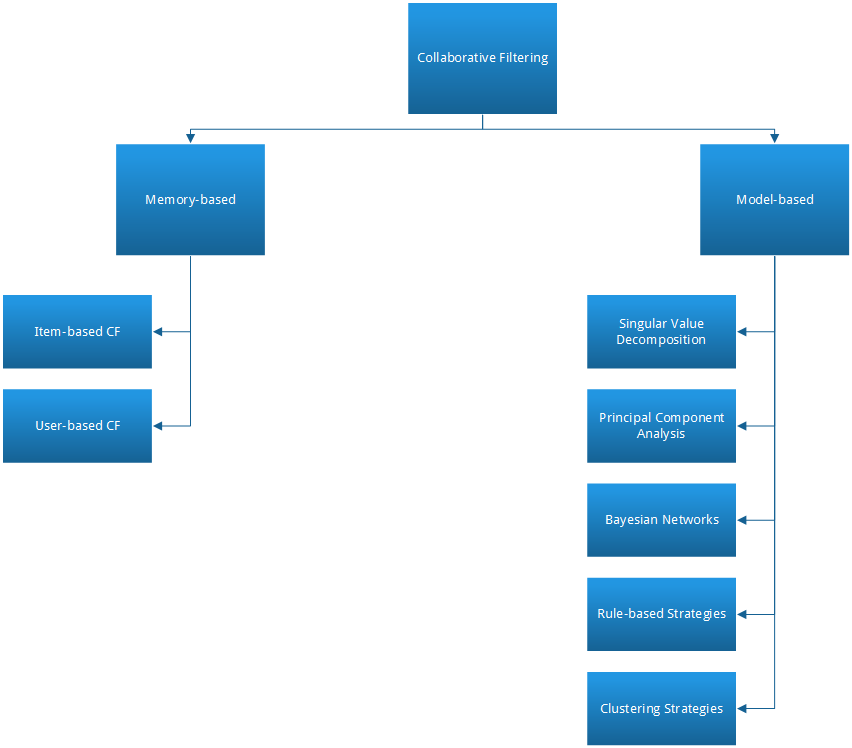
\includegraphics[width=5in]{image/cftaxonomy.png}
    \centering
    \caption[Classification of collaborative filtering techniques]{Classification of collaborative filtering techniques}
    \label{figure:cftaxonomy}
\end{figure}

\textbf{Memory-based Methods}

Memory-based Collaborative Filtering methods utilize the entire user-item database to generate predictions. More formally, the value of an unknown utility $u(c,s)$ for user $c$ and item $s$ is usually computed by taking the weighted average of the utilities assigned by the $N$ most similar users for the same item $s$. The similarity between user $c$ and $c'$, $sim(c, c')$ is used as the weight. The more similar a user $c'$ is to $c$, the more weight is given to the utility $u(c', s)$, and thus, will carry more weight in the prediction for $u(c,s)$.

\begin{equation}
\label{equation:cfratingprediction}
u(c,s) = k * \sum_{c' \epsilon C} sim(c, c') * u(c',s)
\end{equation}

Where k serves as a normalization factor, usually being $1/|C|$. Various approaches have been used to compute the similarity $sim(c, c')$ between the users. Generally these approaches are based on the rating similarities for items both users have rated. The most popular similarity measure is The Pearson Correlation Coefficient. Equation \ref{equation:pearson} shows how to calculate the Pearson Correlation Coefficient between two users $c$ and $c'$, Here $S_{cc'}$ is the set of items the user have in \emph{common}.

\begin{equation}
sim(c, c') = \frac{\sum_{s \epsilon S_{cc'}} (u(c, s)-\bar{u_{c}})(u(c',s)-\bar{u_{c'}})}{\sqrt[•]{\sum_{s \epsilon S_{cc'}} (u(c, s)-\bar{u_{c}})^{2}(u(c',s)-\bar{u_{c'}})^{2}}}
\label{equation:pearson}
\end{equation}

Where $u_{c}$ is the mean utility of user $c$. The Pearson Correlation Coefficient and other similarity measures such as consine based approaches are more commonly known user-based collaborative filtering.\linebreak[2]

Item-based Top-N Recommendation methods calculates the similarity between items instead of users. In these approaches, the historical information is analyzed to identify the relations between items such that a purchase of another item (or set of items) often leads to the purchase of another item. These models are often used since they quickly can recommend a set of items, and have shown to produce recommendation results comparable or better than traditional user-based approaches \cite{Karypis2001}.

The algorithm first computes the $k$ most similar items for each item according to the ratings given by users they both share. Once the most similar items are found, the prediction is then computed by taking the weighted average of the target user's ratings on these similar items.

\begin{equation}
u(c,s) = \frac{\sum_{all similar items, S} (sim(s,S)u(c, S)}{\sum_{all similar items, S}(|s,S|)}
\end{equation}

Items that often are rated similarly by users are considered more similar than items which share few similar ratings. Figure \ref{figure:itemsim} illustrates the process of finding the item-similarities.

\begin{figure}[H]
    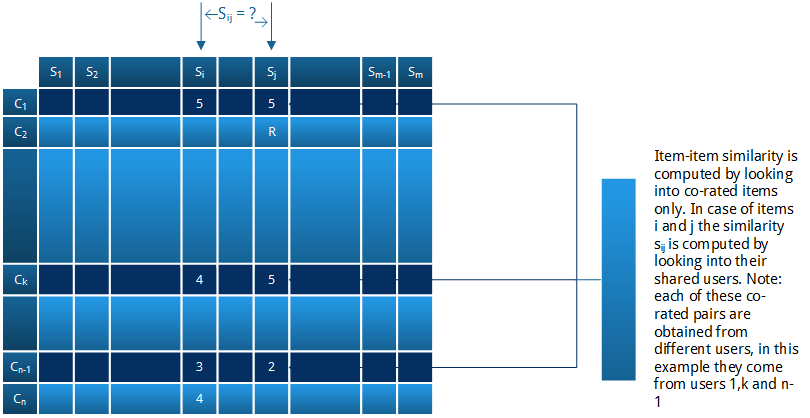
\includegraphics[width=5in]{image/itemsim.png}
    \centering
    \caption[Item-item similarity]{Item-item similarity}
    \label{figure:itemsim}
\end{figure}

There are a number of ways of computing the similarity between items. E.g. by means of cosine-based similarity. In this case, two items are though of as two vectors in an $C$ dimensional user space. The similarity between the items is found by computing the cosine of the angle between the two vectors.

\begin{equation}
sim(s',s) = cos(\vec{s'},\vec{s}) = \frac{\vec{s'} \cdot \vec{s}}{\|\vec{s'}\|^{2} * \|\vec{s}\|^{2}}
\end{equation}

The item similarities are then used to find the Top-N recommendations. Each user has a set of items $S_{c}$ previously rated by the user which we want to compute top-N recommendations for. First, we identify the set $C$ of candidate items recommended items by taking the union of the $k$ most similar items and removing each of the items in the set $S_{c}$ the user already has rated; then calculate the similarities between each item of the set $C$ and the set $S_{c}$, using only the $k$ most similar items for each item in $S_{c}$. The resulting set of items in $C$ are sorted in descending order of similarity and will be the recommended as the item-based Top-N list \cite{Karypis2001}.\newline

\textbf{Model-based Methods}

As the name implies, Model-based approaches provide recommendations by first developing a model of the user ratings, which is then used to make predictions. These algorithms develop a model of user ratings rather than identify a neighborhood of similar users or items. These models can be built using various strategies, such as Singular Value Decomposition (SVD), Principal Component Analysis (PCA), Rule-based Strategies, Clustering Strategies. 

Latent factor models is probably the most representative approach. Latent factor models transform both items and users to a latent factor space. The latent factor space tries to explain the ratings by characterizing both items and users on factors automatically inferred from the data. The most popular latent factor models are based on matrix factorization techniques \cite{Koren2009}.

The main idea behind matrix factorization is just as its name implies, factorize a matrix, finding two or more matrices such that when you multiply them you get back the original matrix. Matrix factorization can be used to discover latent factors underlying the interactions between the users and items. These factors \emph{explain} how a user rates an item (i.e. that a user would give high ratings to a certain shirt if he likes the brand, or if the color is nice). If we can discover these factors, we should be able to predict a rating with respect to a certain user and a certain item based on the correlation between their factors.

A matrix factorization model map both users and items to a joint latent factor space of dimensionality $f$, where $f$ is the number of latent factors. The number of latent factors are usually determined by using a hold-out dataset or cross-validation by evaluating the prediction error experimenting with different values. It is also worth mentioning that this in some ways can be seen as a trade-off between model building complexity and accuracy as having more features makes the model building more expensive. Each user $c$ is associated with a vector $p_{c} \epsilon \mathbb{R}^{f}$, and each item $s$ is associated with a vector $q_{s} \epsilon \mathbb{R}^{f}$. Giving us a matrix Q containing the user factors and a matrix P containing the item factors as exemplified in Figure \ref{figure:matrixdecomp}.

\begin{figure}[H]
    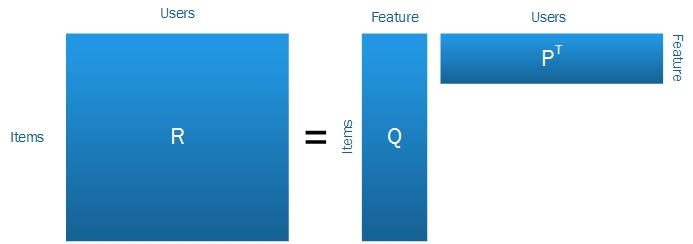
\includegraphics[width=5in]{image/matrixdecomp.jpg}
    \centering
    \caption[Matrix decomposition of the rating matrix $R$]{Matrix decomposition of the rating matrix $R$}
    \label{figure:matrixdecomp}
\end{figure}

User-item interactions are modeled as inner products in that space. For a given item $s$, the elements of $q_{s}$ measures the extent to which the item posessess those factors, positive or negative. Likewise, for a given user $c$, the element $p_{c}$ measures the extent of interest that user has in items that are high on the corresponding factors. The resulting dot product $\hat{u(c,s)}$ captures the overall interest of the user in the characteristics of the items.

\begin{equation}
u(c,s) = p_{c}^{T}q_{s} = \sum_{k=1}^{f} q_{sk}p_{kc}
\end{equation}

The problem then, is to discover the user factor matrix $P$ and the item factor matrix $Q$ such that their product approximates the original rating matrix $R$.

\begin{equation}
R \approx Q \times P^{T} = \hat{R}
\end{equation}

To learn the factor vectors the system minimizes the regularized square error on the set of known rating $K$.

\begin{equation}
\label{equation:minimize}
min_{q, p} = \sum_{(c,s)\epsilon K} (u(c,s) - p^{T}_{c}q_{s})^{2} + \lambda ( \Vert q_{s} \Vert ^{2} + \Vert p_{c} \Vert ^{2})
\end{equation}

However, it is important to remember that our goal is generalize beyond the observed ratings, in a way that we can predict future unknown ratings. The system should therefore avoid overfitting the data by regularizing the learned parameters, whose magnitudes are penalized. $\lambda$ controls the extent of regularization, and much like $f$, often determined by cross-validation. Two possible approaches to minimizing Equation \ref{equation:minimize} is to use Stochastic Gradient Descent or Alternating Least Squares \citep{Koren2009}.

Consider the following example where we have the following rating matrix R shown in Table \ref{table:ratingMatrix} containing the rating of four users $C$ for four items $S$, giving us a $C \times S$ matrix with explicit ratings on a scale from 1 to 5.

\begin{table}[!htbp]
\centering
\begin{tabular}{|c|c|c|c|}
\hline
5.00    & 5.00  & 2.00 & -    \\ \hline
2.00    & -     & 3.00 & 5.00 \\ \hline
 -      & 5.00  & -    & 3.00 \\ \hline
3.00    & -     & -    & 5.00 \\ \hline
\end{tabular}
\label{table:RatingMatrix}
\caption{Rating matrix R ($C \times S$)}
\end{table}

Given that $f = 3$, we might end up with the following matrix $P$ and $Q$

\begin{table}[!htbp]
\centering
\begin{tabular}{|c|c|c|}
\hline
1.81    &1.62   &0.74\\ \hline
2.66    &1.71   &-1.08\\ \hline
1.73    &-0.23  &0.78\\ \hline
3.16    &-0.24  &0.90\\ \hline
\end{tabular}
\label{table:ItemFeature}
\caption{User factor matrix $P$ ($C \times f$)}
\end{table}

\begin{table}[!htbp]
\centering
\begin{tabular}{|c|c|c|c|}
\hline
1.12    &   1.49    &   0.48\\ \hline
1.31    &-0.52  &0.59\\ \hline
1.13    &0.67&  -0.52\\ \hline
1.39    &0.05&  0.45\\ \hline
\end{tabular}
\label{table:UserFeature}
\caption{Item factor matrix $Q$ ($S \times f$)}
\end{table}

Giving us the following rating prediction matrix $\hat{R}$

\begin{table}[!htbp]
\centering
\begin{tabular}{|c|c|c|c|}
\hline
4.79    &5.01   &1.97   &3.61 \\ \hline
1.97    &1.96   &2.85   &4.80 \\ \hline
2.75    &4.71   &1.40   &2.94 \\ \hline
2.93    &3.30   &2.74   &4.78 \\ \hline
\end{tabular}
\label{table:PredictionMatrix}
\caption{Rating prediction matrix $\hat{R}$}
\end{table}

As you can see the values of known ratings in Table \ref{table:ratingMatrix} are fairly similar to the corresponding ratings in the rating prediction matrix.

\subsubsection{Hybrid approaches}

A term \emph{hybrid recommender systems} is used to describe any recommender system that combines multiple recommendation techniques together to provide recommendations. Burke et. al. \cite{Burke2002} identified seven different classes of hybrid recommender systems:

\begin{itemize}
\item Weighted: The score of different recommendation components are combined numerically.
\item Switching: Switching between recommender systems depending on the situation.
\item Mixed: Recommendations from different recommenders are presented together.
\item Feature Combination. Features derived from different knowledge sources are combined together and given to a single recommendation algorithm
\item Feature Augmentation: One recommendation technique is used to compute a feature or set of features, which is then part of the input to the next technique.
\item Cascade: Recommenders are given strict priority, with the lower priority ones breaking ties in the score of the higher ones
\item Meta-level: One recommendation technique is applied and produces some sort of model, which is then the input by the next technique
\end{itemize}

Most commonly hybrid systems are built by combining collaborative and content-based methods in an attempt to mitigate the limitations the approaches suffer individually. Adomavicius and Tuzhilin \cite{Adomavicius2005} lists the following approaches to building hybrid recommender systems:

\begin{itemize}
\item Implementing the systems separately and combining their predictions
\item Incorporating content-based characteristics into a collaborative approach
\item Incorporating collaborative characteristics into a content-based approach
\item Constructing a general unifying model that incorporates both content-based and collaborative characteristics
\end{itemize}

\subsubsection{Recommender System Challenges}

\textbf{Scalability}

As the number of existing users and items blow up, traditional CF algorithms suffer serious scalability problems. The model building phase of \emph{Traditional} collaborative filtering methods have a complexity of O(MN) where $M$ is the number of users and $N$ is the number of items. For systems with millions of users and items, even a complexity of n is too large. Another fundamental issue is how to embed the core recommendation techniques in real operational systems and how to deal with massive and dynamic sets of data produced by the interactions of users with items. Recommender systems are expected in many cases to provide rapid recommendations online, it is therefore also important to consider how fast the system provides recommendations.

Better scalabiltiy and improved accuracy make the item-item collaborative filtering approaches more favorable in many cases. The computational complexity of item-to-item based algorithms are up to two orders of magnitude faster than traditional user-based algorithms \cite{Deshpande2004}. Dimensionality reduction techniques such as SVD can deal with the scalability by providing more compact representations and quickly produce good recommendations. However, most dimensionalty reduction techniques must undergo expensive matrix factorization steps.\newline
\textbf{Sparsity}

In practice, many recommender systems deal with very large item collections. This means that the number of ratings obtained is usually very small compared to the number of ratings that it needs to predict. Efficient prediction of ratings from a small number of examples is therefore important. The \emph{reduced coverage} problem occurs when the number of users' rating may be very small compared to the number of items. This may lead to that the recommender is unable to provide recommendations for a large portion of the items. \emph{Neighbour transitivity} refers to the problem in which users with similar tastes may not be identified due to a lack of co-rated items, making collaborative filtering futile, since it relies on comparing users to predict unknown ratings. \linebreak[4]

\textbf{Cold-start}

Conceptually, the cold-start problem can be viewed as a special instance of the sparsity problem, where most elements in a certain row or column are zero. The cold-start problem further emphasizes the importance of the sparsity problem. Whenever a new user or item enters the system, it is difficult to find similar ones as there is little or no information available. New items can therefore not be recommended until they have been recommended by a substantial amount of users. Similarly, giving \emph{good} personalized recommendations to new users based on a few ratings is difficult, since it does not give a good overall picture of a users tastes and preferences. These problems are known as the \emph{cold-start user} and \emph{cold-start item} problems. \linebreak[4]

\textbf{Shilling attacks}

In recommender systems where everyone can give ratings, people may give lots of positive ratings to their own items and negative ratings to their competitors. It is often necessary for collaborative filtering systems to introduce precautions to discourage such kind of manipulation. \linebreak[4]

\subsubsection{Terminology}

%TODO - Any more RS related terminology that needs explaining?

\textbf{Explanations / Transparency}

Tintarev et. al. \cite{Tintarev2007} lists seven roles a that can be played by explanations in recommender systems:

\begin{itemize}
\item Transparency: Explaining how the system works
\item Scrutability: Allowing the users to tell the system it is wrong
\item Trust: Increasing user confidence in the system
\item Effectiveness: Help users make good decisions
\item Persuasiveness: Convince users to try or buy
\item Efficiency: Helping users to make decisions faster
\item Satisfaction: Increasing the ease of use or enjoyment
\end{itemize}

In collaborative filtering systems the explanations is of the form "Other users similar to you liked this item", while in content-based style explanations, the item's attributes which most affected the item to be recommended to the user are illustrated. For example, in a fashion recommender, an explanation may be of the form "This shirt was recommended because it's a Ralph Lauren who you seem to like".

\subsection{System Cold-start Handling}

%Can the different approaches be classified? E.g. 3 main categories of approaches
    %Initial categorization
        %Interview process
        %Hybrid approaches
        %Key figures / Seed users
        %Filterbots
        %Trust-aware / Trust propagation

In the literature, the term cold is used about an object in a system, or a
whole system, which is new \cite{Schein2002, Park2006}. Cold-start scenarios in recommender systems are
situations in which little/no prior events, like ratings or clicks, are known
for certain users or items. The cold-start problem can be divided into three sub problems:

\begin{itemize}
  \item \emph{Cold-start system}: A situation where we only have new users and
  little or no ratings for the items.

  \item \emph{Cold-start item}: The problem of recommending items that are new
  to the system, which have not received any ratings.

  \item \emph{Cold-start user}: The problem of giving accurate recommendations
  to a user who is new to a recommender system.
\end{itemize}

For example in a scenario where the average item in an item collection have 5 000 ratings, a new item with only 5 ratings would be considered a \emph{cold-item}. Likewise, in a recommender system where the average user has rated 25 items, a user who only has rated 2 items, would be considered a \emph{cold-user}.\linebreak[4]

The cold-start system problem is mainly a collaborative filtering problem, and
can be seen as a combination of the cold-start user and cold-start item problem
where the majority of the users are new to the system and have expressed few
preferences, resulting in a very sparse user-item matrix, rendering traditional collaborative-filtering methods futile. Most traditional algorithms only work effectively in environments where the datasets has high information density. In fact, in extreme cases, when data
is very scarce, simple non-personalized recommendations based on global
averages can outperform collaborative-filtering algorithms \cite{Park2006}. The reason why the cold-start system problem is not so evident in content-based systems is due to \emph{User Independence}, meaning that the system only exploits ratings provided by the active user to build her profile. Instead, collaborative filtering methods need ratings from other users to find the "peers" of the active users.

In content-based systems, new items can easily be
recommended using the content information of the item, making it a popular
solution to the \emph{cold-start item} problem. This problem is more
severe in collaborative-filtering systems where items are only recommendable if
they have been rated by substantial amount of users. New items will therefore not be
recommendable before multiple users somehow stumble upon the new item while
e.g. browsing the item collection, unless additional measures are taken to
solve this problem. To \emph{solve} the new-item problem, there are two commonly used (simple) solutions often used in E-commerce websites:

\begin{itemize}
\item Advertising at the front-page of the website, putting the new
items in an eye catching position. This solution, however, may this result in
that some users, which don't like these new items, might leave the website.
\item Requesting the user to choose one or more of his/hers categories while
registering for the site, and recommend items from the selected categories.
This approach however, requires active user involvement and complicates the
sign up process. Many users might chose not to give up any
personal interest information, thus the user group covered by this solution could end up not being large enough.
\end{itemize}

The cold-start user problem is present both in content-based and
collaborative-filtering systems. Collaborative Filtering is based on the idea that like-minded users have similar tastes and
preferences. A new user therefore poses a challenge to a CF recommender, since
the system has no knowledge about the preferences of the new user, and can
therefore not provide any personalized recommendations. The system must therefore acquire some
information about the new user before it can start making personalized recommendations. In a typical domain, for example in the domain of books, the number of items is very large (in the order of tens of thousands) while the number of items rated by every single user is in general small (in the order of dozens or less). This means that it is very unlikely two random users have rated any items in common and hence they are not comparable. The system will therefore most likely struggle to find users with tastes that are \emph{truly} similar to the target user. Similarly, in content-based systems, the lack of ratings given by the target user, means that the target user will have a limited
content-profile, since the users content profile is constructed using content-information from his/hers rated items. In both cases, recommendation quality is most likely bound to suffer.\linebreak[4]

This section will present a few different solutions to the cold-start problem, focusing mainly on \emph{complete} solutions to the cold-start problem.

\subsubsection{Trust Aware Recommender Systems}

One promising direction to solve the cold-start problem is the incorporation of a trust network. A trust network can significantly help alliviate the cold-start user problem, primarily since the trust statements between users can be propagated and aggregated, and consequently connect more people and products. By making clever connections in the trust network, newcomers can immediately gain access to a wide range of connections.

Due to the popularity of social networks such as Facebook, more and more
researchers turn to incorporate the social relationships (e.g. trust) of users
to help complement users’ preference in addition to item ratings, in order to overcome the limitations of existing recommender systems. For example, when looking for movie recommendations we often turn to our friends which we share a similar taste in movies with. Trust can be defined as: "believe in the reliability, truth, or ability of", and in the context of recommender systems a trusted user would be a user you trust to provide you with good recommendations. E.g. in the case of the Epinions dataset \cite{Epinions}, users can explicitly state whether they trust or distrust a user [1, -1], i.e. reviewers whose reviews and ratings they have consistently found to be valuable or reviewers which they find consistently offensive, inaccurate or not valuable. In decentralized environments where everyone is free to create content and there
is no centralized quality control entity, evaluating the quality of the content becomes an important issue. This phenomenon can be observed in online
marketplaces such as E-bay where users can create "fake" auctions and in peer-to-peer networks where peers can enter corrupted items. In these environments, it is often a good strategy to delegate the quality assessment task to users themselves. E.g. \emph{Ebay.com} allows users to express their level of satisfaction after every interaction with another user. Trust relationships of users are often employed in order to correlate more potential raters for the active users who require recommendations \cite{Massa2004, Massa2007}. Massa et. al. \cite{Massa2004} also show that some of the weaknesses of recommender systems such as data sparseness and their susceptibility to shilling attacks could be alleviated by incorporating trust.

% The formals
In \cite{Massa2004}, Massa et. al. proposes a Trust-Aware recommender system architecture.
To capture all the trust statements we need a $CxC$ matrix, where $C$ is the number of users, since each user is allowed to express a trust value in every other user. This matrix will make up our trust network among the users. If $u$
trusts $v$, then there is a value $t_{u,v}$ for this trust which is a real
number in $[0,1]$. Zero means no trust and one means full trust. This additional information can be organized in a trust network and a \emph{trust metric} can be used to predict the trustworthiness of other users as well (for example, friends of friends). The idea here is to not search for similar users as CF does but to search for trust-able users by exploiting trust propagation over the trust network. The items appreciated by these users are then recommended to the active user.

% Web of Trust - Figure explanation
Consider the example shown in Figure \ref{figure:weboftrust}. User $A$ has issued a trust statement in $B$ and $C$; hence
$B$ and $C$ are in the web of trust of $A$. Using these explicit trust statements, it
is possible to predict trust in unknown users by propagating trust, making it
possible to infer something about how much user $A$ could trust $D$.

\begin{figure}[H]
    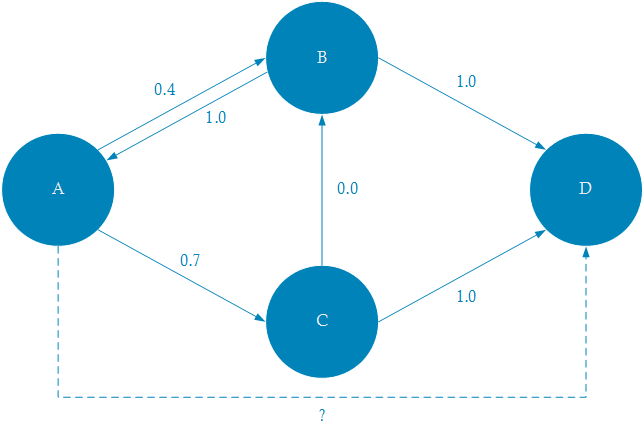
\includegraphics[width=2in]{image/webofTrust.png}
    \centering
    \caption[Trust Network]{Trust Network. Nodes are users and solid edges are trust statements. The dotted edge is one of the undefined and predictable trust statements (Adopted from \cite{Massa2004})}
    \label{figure:weboftrust}
\end{figure}

In addition to the trust network we will also have a rating matrix of size $CxS$, where $S$ is
the number of items. This rating will not differ from a standard rating matrix, which are used in traditional collaborative filtering systems. The value $u(c,s)$, is the rating given by user $c$ to item $s$, the rating scale may differ from system to system.

% Architecture
The systems takes as input the trust network and the ratings matrix and
produces, as output, a matrix of predicted ratings that the users would assign
to the items. Figure \ref{figure:trustarchictecture} shows a conceptual
overview of the trust-aware recommender system architecture.

\begin{figure}[H]
    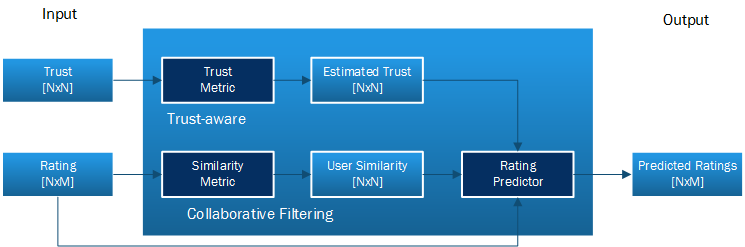
\includegraphics[width=5in]{image/trustawarearchitecture.png}
    \centering
    \caption[Trust-Aware Recommender System Architecture]{Trust-Aware
    Recommender System Architecture (Adopted from \cite{Massa2004})}
    \label{figure:trustarchictecture}
\end{figure}

The \emph{Trust Metric} module takes the trust network as input, and exploits
trust propagation in order to predict, for every user, how much she could trust
other users. Trust metrics can either be local and global. Global trust metrics
produces an estimated trust matrix with all the rows equal, meaning that the
estimated trust in a certain user (column) is the same for every user (row). A
simple local trust metric could e.g. for each user assign to every other user a
predicted trust based on her minimum distance from the source user. More
sophisticated ones could also be employed. If we again consider Figure
\ref{figure:weboftrust}, we could employ a local trust metric where the
predicted trust is based on the minimum distance from the source user. If we
set the maximum propagation distance $d$, a user at distance $n$ from the
source user will have a predicted trust value of:

\begin{equation}
t_{u,v} = (d-n+1)/d
\end{equation}

Giving users not reachable within the maximum propagation distance a trust of
$0$. Using user $A$ as the source user, the users at distance $1$ ($B$ and $C$)
would get a trust value of $(4-1+1)/4 = 1$, while the user at distance 2 (D)
would get a predicted trust value of $(4-2+1)/4 = 0.75$. Meaning that we will
have a linear decay in trust based on the distance from the source user.

Massa et. al. \cite{Massa2007} experimented with both local and global trust
metrics. They used the PageRank algorithm as a global trust metric. PageRank
tries to infer the authority of every single user by examining the structure of
the network. The algorithm follows a simple idea: if a link from user $A$ to user
$B$ represent a positive vote casted by $A$ to $B$, then the global rank of a page
depends on the number (and quality) of the incoming links. The trust values
assigned by users to users are used to predict the trustworthiness of unknown
users. Their findings, not surprisingly, indicate that Global Trust Metrics are
not suited for the task of finding good neighbors, especially for providing
personalized recommendations, but is more suited to applications such as \emph{Ebay.com} to find untrustworthy users. As a local trust metric they used MoleTrust, which is a depth-first graph walking algorithm with a tuneable trust horizon
which allowed them to experiment with different propagation distances. They found trusted users to be good predictors. For the cold-start users they achieved a MAE of 0.674 when looking at friends of friends, compared to traditional collaborative filtering which scored 1.094. The difference is very high, and particularly relevant as it is important for recommender systems to generate personalized recommendations as soon as possible for new users, so that these users appreciate the system and keep using it.

The \emph{Similarity Metric} module computes the user similarities, this is one
of the standard steps of any traditional collaborative filtering technique,
user similarities can be found e.g. by using the Pearson Correlation
Coefficient. The intuition is that, if a user rates in a similar way to another
user, then her ratings are using for predicting the ratings for that users.

The \emph{Rating Predictor} can use the neighbors from the user similarity
matrix, the estimated trust matrix or a combination of both in order to
calculate the predicted ratings.

% Using a Trust Network to Improve Top-N Recommendation


Jamali et. al. \cite{Jamali2009} propose two different methods for getting
around the cold-start user problem using a trust network. Their first approach called \emph{Random Walk} only utilize the trust network to provide recommendations. Starting from the active user $u$, we perform a random walk on the trust network. Each random walk stops at a certain user. Then the items rated highly by that user
will be considered as recommended items, ordered according to the ratings
expressed by that user. Several random walks are performed to gather more
information and compute a more confident result. The estimated rating of each
item is the average of ratings for that item over all raters considered. At the
end, we output items with the highest estimated rating as top-N recommended
items. Their second approach called \emph{Combined Approach} uses both user-user similarities and the trust network to provide recommendations. In this approach we compute the top $K$ trusted users in the network and rank
the items rated by these trusted users to compute top-N recommended items. The top $K$ trusted users can either be found by
\emph{Breadth First Search} or \emph{Random Walk in the social network}. We use the collaborative filtering approach to compute another set of top-N recommended items. Finally, we merge these two lists to produce a combined list of top-N recommended items. Items returned by CF is denoted as $CF_{u}$, while the items returned by Trust-based approach are denoted $TR_{u}$.

\begin{equation}
 \hat{u}(c,s) =
  \begin{cases}
   \frac{u_{tr_{c,i}}+u_{cf_{c,i}}}{2}     & i \in TR_{u};i \in CF_{u}         \\
   \hat{u_{tr_{c,i}}}                      & i \in TR_{u};i \not \in CF_{u}    \\
   \hat{u_{cf_{c,i}}}                      & i \in CF_{u};i \not \in TR_{u} 	\end{cases}
\end{equation}

The top-N items with the highest value of $\hat{u}(c,s)$ will be returned as the top-N recommended items. The authors also experimented with weighted averaging in the case where the item appear in both $TR_{u}$ and $CF_{u}$.

The top-N items with the highest value of $\hat{u}(c,s)$ will be returned as the top-N recommended items. The authors also experimented with weighted averaging in the case where the item appear in both $TR_{u}$ and $CF_{u}$. Their approaches showed great improvements in recall for cold-start users,
improving the performance by 50\% over standard CF methods. The main improvements however, are the coverage of the trust-based approaches, while still maintaining the same or even slightly better precision than the standard CF methods.

% Trust-aware Recommender Systems + Trust-Aware Collaborative Filtering for Recommender Systems
% Article Comments:
%   Requires user involvement (explicitly express trust) - is this a acceptable?

%Massa et. al. \cite{Massa2004, Massa2007} propose using trust information
%explicitly expressed by the users. Users are allowed to state how much they
%consider every other user trustworthy that, in the context of recommender
%systems, is related to how much they consider the ratings provided by a certain
%user valuable and relevant.

% Alleviating the Sparsity Problem of Collaborative Filtering Using Trust Inferences
% Article Comments:
%   - Pretty good general model for dealing with sparsity
%   - Requires no additional information such as product details, demographic information about userstrus


Papagelis et. al. \cite{Papagelis2005} proposed to alleviate sparsity using
trust inferred from user-user similarity. This approach does therefore not require users to explicitly express their trust in other users, unlike the approaches described above, the trust information is inferred from the underlying social network of the rating matrix. Their approach is based on the assumption that the more similar two users are, the greater their established trust would be considered.

\begin{figure}[H]
    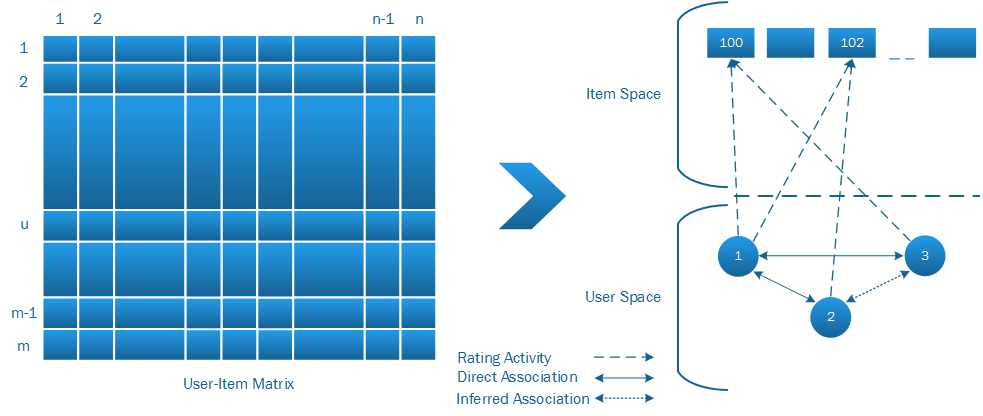
\includegraphics[width=5in]{image/trustnetwork.png}
    \centering
    \caption[Underlying Social Networks in Recommender Systems]{Underlying Social Networks in Recommender Systems}
    \label{figure:cfsocialnetwork}
\end{figure}

Due to the number of ratings that exist in recommendation systems, underlying
social networks are very sparse. There are cases in which insufficient or loss
of information is detrimental for the recommendation algorithms. Consider
Figure \ref{figure:cfsocialnetwork}, classic CF will associate only the users
which have co-rated an item (User $1$ and $2$ and user $1$ and $3$). To deal
with the problem of a sparse social network, it is possible to infer trust
between a source user $S$ and a target user $T$ through an intermediate user
$N$ (User $2$ and $3$ are connected through the intermediary user $1$), as
shown by the \emph{Inferred Association} arrow. According to this process,
trust is propagated in the network and associations between users are built,
even if they have no co-rated item. Trust paths can be of variable length,
depending on the number of associations that one needs to traverse in order to
reach the target user.

% Trust-paths
For example, if the trust $t_{(1,2)} = 0.7$ based on 5 co-rated items
and $t_{(1,3)} = 0.35$ based on 2 co-rated items, then the trust
between user $2$ and $3$ through $1$ is, $\frac{0.7*5}{5+2} + \frac{0.35*2}{7} = 0.6$.

In order to express the subjective notion of trust, the authors set up a
confidence model that is assigned to each direct association of the network
that expresses the reliability of the association. Confidence is related to the
number of co-rated items between two users. The confidence scores are all
expressed in relation to the most confident association for each user.

\begin{equation}
c_{(s,t)} = \frac{n(I_{s} \cap I_{t})}{n(I_{s} \cap I_{u_{MAX_CONF}})}
\end{equation}

Using the above example, assuming that the maximum number of co-rated items
user $1$ has with any user is 7, $c_{(1,2)} = \frac{5}{7}$.

% Results/Findings
The authors achieved improved accuracy for all sparsity levels. With a sparsity
level of $99.9\%$ the 2-HOP CF (friend of friends) increased the MAE
performance by $17\%$ over standard CF methods.

%TODO - READ: A Matrix Factorization Technique with Trust Propagation for Recommendation in Social Networks
%Jamali et. al. propose a technique for incorporating trust using matrix factorization, called SocialMF.
%Leverage regularization model to fusing the one mode data by minimizing the gap between the taste of a user and the taste of her trusted friends
%In their model, the users which have not expressed any ratings feature vectors will be learned to be close to their trusted neighbors.

Victor et. al. \cite{Victor2008} points out that cold-start users not only have expressed few ratings, but also typically have expressed trust in few users. In order for trust-aware recommenders to help cold-start users they need to have expressed trust in atleast one user. But choosing who to connect to is often a difficult task. To help cold-start users find trusted users, Victor et al. propose using key figures or mavens, frequent raters and connectors (users with many trust connections). By connecting to these key figures, cold-start users shown a significant increase in coverage while still maintaining good accuracy. They also show that connecting to key figures are more beneficial to a cold-start user than connecting to a random user.

\subsubsection{Filterbots}

% Na¨ıve Filterbots for Robust Cold-Start Recommendations

Park et. al. \cite{Park2006} propose using filterbots to improve the cold-start
performance of collaborative filtering methods. Their filterbots are a varition of RipperBots, described in detail in \cite{Good1999}. A filterbot is an automated agent that rates all or most items using information filtering (IF) techniques. The filterbots injects psuedo
users or bots into the system. These bots rate items algorithmically according to item features and user profiles. For their movie recommendation systems the authors used 7 global bots which rates movies based on average item rating, a critic bot that generates ratings based on the average critic (pre-selected users) ratings, an award bot that generates rating based on the awards a movie has won, and so on. These ratings generated by these bots are injected into the user-item matrix along with actual user-item ratings. Standard CF algorithms are then applied to generate
recommendations.

Their approach clearly demonstrated better robustness to all three cold-start situations than standard item-based
and user-based collaborative filtering. The improvements were most evident on
the datasets with a high degree of sparsity.

% Discussion

\subsubsection{Wisdom of the better few / Seed users}

% Wisdom of the Better Few: Cold Start Recommendation via Representative based Rating Elicitation

Liu et. al. \cite{Liu2011} propose an approach in which they elect a few
representative users and items. The representative set should represent a set
of active users or items who well represent the entire population but with
little taste overlap. In their approach they wish to find a rank-k
factorization of the form $Y \approx XR$ or $Y \approx CX$ where $X$ is a
loading matrix consisting of free parameters and $R$ and $C$ which is the
component matrix consisting of actual rows or columns from $Y$. The
representative users and items are found using dimensionality reduction
techniques by reducing the column space of the rating matrix from $m$ to $k$.
And then applying basis selection based on the maximum-volume principle to
select the $k$ most representative users or items. In order to be able to
recommend new items to the users it must first be rated by the $k$
representative users, likewise for new users to be rated they need to rate the
$k$ most representative items. Their method therefore easily allows new users
and items to be \emph{folded in}.

\subsubsection{Intelligent Selection / Interview Process}\mbox{}\\

%My though behind including these articles:
%Use e.g. a tinder like interface and ask the user to like/dislike 15 items when first logging in

\begin{chapquote}[30pt]{Vanessa Redgrave}
  "Ask the right questions if you're going to find the right answers"
\end{chapquote}

% Getting to Know You: Learning New User Preferences in Recommender Systems

As pointed out by Rashid et. al. \cite{Rashid2002}, the most direct way of
acquiring information for use in personalized recommendations from a new users
is to present item for the user to rate. However, they argue that the system
must be careful to present useful items to garner information. A food
recommender should probably not ask whether a new user likes vanilla ice cream
since most people like vanilla ice cream. Therefore, knowing that a new user
likes vanilla ice cream tells you very little about the user. The choice of
what questions to ask a new user, then, is critical. The authors performed a
study of different item selection strategies that collaborative filtering
recommender systems can use to learn about new users. They presented the users
with a questionnaire with items asking them to rate/select the ones they like.
Their strategies can be divided into five classes, which they evaluated based on user effort and accuracy:

\begin{itemize}
\item \emph{Random:} strategies: Strategies that avoid bias in the presentation
of bias
\item \emph{Popularity:} Select among the top N items where the probability
that an item is selected is proportionate to the items popularity.
\item \emph{Pure entropy:} Present the items with the highest entropy that the
user has not seen
\item \emph{Balanced strategies:} A balanced approach combining both popularity
data and entropy.
\item \emph{Personalized:} As soon as some information is known about a user,
present items specifically tailored to that user using e.g. item-item
similarity
\end{itemize}

The authors found Popularity and balanced strategies to perform the best. Their recommendation for an e-commerce recommender is to start recommending the most popular items, rather than the highest rated ones, and then use item-item strategies to personalize the recommendations as quickly as possible. This study was later extended by Rashid et. al. \cite{Rashid2008} where they
more closely examined information theoretic strategies for item selection. In the article they introduced three new strategies, which again was evaluated based on user effort and accuracy:

\begin{itemize}
\item \emph{Entropy0}: Entropy Considering Missing Values
\item \emph{HELF:} Harmonic mean of Entropy and Logarithm of Frequency
\item \emph{IGCN:} Information Gain through Clustered Neighbors
\end{itemize}

The authors point out that approaches like popularity is likely to worsen the \emph{prefix-bias}, meaning that popular items garner even more evaluations. The accuracy differences between the approaches is fairly small, IGNC performed the best closely followed by Entropy0 and Popularity. However, the expected utility of the profiles built using popularity is much lower than the information theoretic approaches.\linebreak[4]

% User effort vs. accuracy in rating-based elicitation
The question then, is how many items you should ask a user to rate. Cremonesi et. al. \cite{Cremonesi2012} performed a set of experiments where
they looked at the trade-off between user-effort and accuracy. More
specifically, how many ratings are enough to provide good quality
recommendations to new users? The authors conclusion is that between 5 and 20
ratings are optimal for the movie domain. They concluded that 10
ratings is \emph{enough}, but that this number depends on the recommendation method
and the dataset used.

\subsubsection{Hybrid Methods}

%TODO - Add some fancy math, wait until matrix factorization intro is in place (so we do not mess up notations)
%TODO - Find some sweet cf articles incorporating demographic information

Another line of search for solving the cold-start problem is to utilize features of items and users. The content features can be used to capture the similarities between users and items, thus reducing the amount of data required to make accurate predictions. User data that may be collected typically includes age, gender, nationality, marital status, income, educational level and occupation. Item data could e.g. be the price of a product, title, description, editorial ratings and so. The idea is that people with a more common background share a more similar taste than someone with a random background, and therefore good recommendations can be made as long as we know something about the new user’s background. 

This section will present some latent factor models presented recently proposed that incorporate both user/item features in addition to user-item interactions. In Matrix factorization methods, the regularization is mostly based on a
zero-mean Gaussian prior on the factors, we refer often referred to as ZeroMean. However in the following models the dyadic response matrix $Y$ is estimated by a latent factor model such that $Y \approx U^{T}V$, where the latent factor matrices, $P$ and $Q$, are estimated by regression such that $P \approx FX$ and $Q \approx MZ$. $X$ and $Z$ denote user attribute and item feature matrices, and $F$ and $M$ are weight matrices learned by regression. The main difference between the following methods is how they estimate these weight matrices.

% Regression-based Latent Factor Models

Agarwal et. al. \cite{Agarwal2009} propose a class of latent factors models called regression-based latent factor model (RLFM) that incorporates both user/item features and past interaction data into a single model. Their approach utilizes features of items and users as the
prior distribution for latent profiles in matrix factorization. Regularizing latent factors through regression has important consequences when modeling sparse dyadic data. For users/items with little data, one obtain reliable factor estimates by using the regression estimates as a fallback. This allows the model to effectively deal with both cold start and warm start situations. Their method assumes a Gaussian prior, but replaces the zero mean with a feature-based regression, thus it simultaneously regularizes both user and item factors through known features. Users and items are anchored around a global feature-based one where profiles are constructed by estimating deviations from the global ones in a smooth fashion. The deviation depends on the amount of information available, e.g. items/users with sparse data are aggressively "shrunk" to the global one. New items and users start out with profiles based on their known features that gets refined smoothly with the availability of more data.

Their model outperformed all other models on both the MovieLens and EachMovie datasets, and their dynamic model in particular significantly outperformed all other models.

% fLDA: Matrix Factorization through Latent Dirichlet Allocation

Agarwal et. al \cite{Agarwal2010} propose a Matrix factorization method to predict ratings in recommender system
applications where a "bag-of-words" representation of item meta-data is natural. Their method regularizes both user and item factor simultaneously through user features and the bag of words associated with each item. The key idea of their method is to let user factors take values in an Euclidean space of existing factorization models, but assign item factors through a richer prior based on Latent Dirichlet Allocation (LDA). The main idea behind LDA is to attach a discrete latent factor to each word of an item that can take $K$ different values ($K$-topics) and produce item topics by averaging the per-word topics in the item. An article where 80$\%$ of the words are assigned to politics and the rest to education would be though of as a political article related to the issue of education. This allows us to model the affinity between user $i$ and item $j$ as $s'{j}\hat{z_{j}}$, where $\hat{z_{j}}$ is the multinomial probability vector representing the soft cluster membership score of of item $j$ to the $K$ different latent topics. 

% Matchbox: Large Scale Bayesian Recommendations
% 	Online algorithm

Stern et. al. \cite{Stern2009} presents a probabilistic model called Matchbox. The system makes use of content information in the form of user and
item meta-data in combination with collaborative filtering information from previous user behavior in order to predict the value of an item for a user. Much like \cite{Agarwal2009} the factors are regularized by incorporating more flexibility in the Gaussian priors through regression on user and item factors. Their model is dynamic, meaning that it allows an item's popularity, a user's taste or user's personal rating scale to drift over time, as well as having the option to be trained incrementally using Assumed Density Filtering (ADF). This means that the value of weight matrices $F$ and $M$ will drift over time, this is accomplished by the addition of Gaussian noise each time step. Inference is accomplished a combination of message passing and expectation propagation.

The authors show that they can achieve state-of-the-art performance when training the model in an on-line manner, which is especially beneficial for dynamic domains where it is important to always have an up to date model. Matchbox was able to train the model for the Netflix Dataset in about 2 hours using 8 cores, meaning that it is able to add up to 14000 ratings per second. These methods also provide quick recommendations, which is important in an online applications, the system was able to generate 2,500,000 recommendations in 0.25s using Approximate KD Trees.

% Learning Attribute-to-Feature Mappings for Cold-Start Recommendations
% 	Model for positive implicit feedback!
% 	Demonstrates usefulness for new-item recommendations
% 	See A. Item Recommendation from Implicit Feedback in the article for implicit feedback recommendations
%	k-NN worked best with MORE features than the linear mapping functions
%	Code can be found at: ismll.de/mymedialite

Gantner et. al. \cite{Gantner2010} propose a method on how to map additional
information such as user and item features to the latent features of a matrix
(or higher dimensional) factorization model. At the core of their approach is a
standard factorization model, optimized to the recommendation task. The
extensions include a mapping function that compute adequate latent
representations for new entities from their attribute representations. This
mapping function could allow new items and users latent features to be found
only based on content-information and further on be used as if they were
normally trained latent features. The training of the factorization model with
a mapping extension consists of the following steps:

\begin{enumerate}
\item Training the factorization model using the data $S$, and then
\item Learning the mapping functions from the latent features of the entities in the training data and their content attributes
\end{enumerate}

The authors use BPR-MF, a matrix factorization model based on the Bayesian Personalized Ranking (BPR) framework as their factorization model. The authors experimented with two different ways of mapping item/user attributes to the factor space (Only attribute-to-feature mapping for items are presented in the article):

\begin{enumerate}
\item k-NN Mapping:	Weighted k-NN regression for each factor. Determine the k-nearest neighbors as the most similar items according to the cosine similarity of the attribute vectors.
\item Linear Mapping: Each item factor is expressed by a weighted sum of the item attributes. Suitable parameters for the mapping function is learned by optimizing the model for the squared error on latent features.
\end{enumerate}

The authors found that linear mapping worked the best, and that their method yields accuracy comparable to state-of-the-art methods.

\subsubsection{A Discussion on the Cold-start Solutions}

\textbf{Trust-aware recommenders}

%Summarize results
Massa et. al. \cite{Massa2007} found trusted users to be good predictors. When looking at directly trusted users they improved the MAE from 1.094 using traditional collaborative filtering to 0.674 for cold-start recommendations. By propagating the trust they were able to drasticly increase the coverage. The average number of directly trusted users were 9.88, while the average number of comparable users using the pearson correlation factor was 160.73. Propagating at a distance of 2 it is possible to reach 399.89 users, increasing it to 3 and 4 respectively it is possible to reach respectively 4,386.32 and 16,033.94 users. Jamali et. al. \cite{Jamali2009} got even better results with their \emph{Trustwalker} approach by combining trust-based and item-based recommendations. Massa et. al. \cite{Massa2004} also argue that it is more useful for a recommender system to ask for one trust statement than asking for one rating for new users.

%How can this be implemented in our system?
Requiring users to explicitly express trust, is not something users necessarily will frown upon. Services like Instagram, Facebook and many others offers a "follow" function to their users, filling their news feeds with content from the users which they have chosen to follow. For Sobazar we imagine that you e.g. could chose to follow people either because they have a good taste in clothes or that you simply are friends, and you want to keep up with what your friends are buying.

%Scalability & Final Verdict
Propagating trust is expensive. The trust propagation must be computed in addition addition to the user-user or item-item similarities, and it therefore scales worse than collaborative filtering methods. Good general model for sparsity and increasing robustness of recommender systems, with the downsides being scalability challenges and the added complexity to the system.\newline

\textbf{Interview Process}

%Summarize results
Rashid et. al. \cite{Rashid2008} got the best results using information theoretic approaches and argues that simpler methods such as most popular is likely to worsen the prefix bias. The authors found Information Gain through Clustered Neighbours (IGCN) to have the best performance overall, which scored 5 out of 5 stars for accuracy, and would be a good candidate to find items for the user to rate.

%How can this be implemented?
Our rational behind including these articles is that we envision a simple "hot or not" tinder like interface to be used to present items to new users when the first log in to the system. And then ask new users that download the app to rate e.g. 10 items when first logging in. It is worth mentioning that the authors of these articles mainly worked on a solution to the cold-start new user problem. The user-effort dimension of their evaluation could also largely be ignored as they made a system for movie recommendations. The implications of this is that a user must have watched a movie, in order to rate it. This is not as important for the fashion domain, as taking a quick look at an item should be sufficient to like/dislike it, so we should give more weight to the accuracy of the system after the interview process than user effort. It is also worth noting that calculating entropy using implicit ratings is tricky, since the rating distribution does not range from dislike to like. We can therefore not find \emph{high-entropy} or \emph{controversial} items which users either tend to like or dislike, as we have no data about items users dislike \todo{Discussion on suitedness of implicit ratings for entropy calculations}. We are also currently constrained to unobtrusively learn user-profiles from the natural interactions of users with the system, meaning that we can not require the user to rate e.g. 10 items before we can start providing recommendations, as this functionality has not been implemented.

%Scalability & Final Verdict
The scalability of the approach is also fairly good. It requires another module in addition to collaborative filtering which is used in the non-personalized step until the user have rated a predetermined amount of items. When enough items have been rated the CF algorithm is used to produce recommendations. We really like this approach as it is simple and elegant. Given that a information theory approach is used this would be a good model for dealing with sparsity, as the number of ratings would sky-rocket in addition to having ratings for a large portion of the item collection (not only limited to the most popular items). The negative aspects of this approach is mainly limited to the fact that it requires active user involvement.\newline

\textbf{Seed users}

In our opinion, this approach is not that suited for our domain, as it fairly dynamic and we are working with a large item collection. For an item to be recommendable it must be rated by all representative users, which is highly unlikely given the size of the item collection itself. E.g. if we have 15 representative users and a spring collection launches containing 6000 items, for all these items to be recommendable these 15 representative users must rate all these items.\linebreak[4]

\textbf{Filterbots}

%TODO - Summarize results
Park et. al. \cite{Park2006} clearly demonstrated the robustness of their Naive Filterbot compared to item-based and user-based approaches in all three cold-start scenarios. The results in \cite{Agarwal2009, Agarwal2010} also shows that the Naive Filterbots performance is very close to the state-of-the-art latent factor models.

%TODO - How can we implement this in our system?
To incorporate filterbots in our system we would first have to define what filterbots we wound want to use. We could e.g. use a Brand-bot that calculates ratings of brands over all users. The rating of a brand is the average rating of the items of the given brand, which then is injected into the user-item matrix. It is worth noting that selecting what bots to add to the system and and coding them would require some engineering effort, and involve some testing to validate your bots.

%TODO - Scalability & Final Verdict
Park et. al. \cite{Park2006} claim that the added computational complexity of adding seven global bots is almost negligible. The downside of this approach is the additional engineering effort required and the fact that it's performance is not on pair with the more sophisticated latent factor methods.\newline

\textbf{Hybrid recommenders}

%TODO - Summarize results

Latent factor models are currently the main paradigm within the recommender system field and are currently considered the state-of-the-art recommendation methods. The hybrid methods achieved state-of-the-art performance as well as having good fallback methods based on user and item features to solve the cold-start problem.

%TODO - How can we implement this in our system?
To implement these recommenders we would first have to select and extract user-features from Facebook and item-features from our item database. Another concern of ours is that our dataset is currently to small for latent factor methods, and is therefore likely to produce sub-optimal results.

%TODO - Scalability & Final Verdict
%	Which of the models are online?
As most latent factor models, model building is expensive. Matchbox and RLFM have to option of being trained online, which should further could increase the cold-start performance, as the model always will be up to date. Latent factor models are also known to provide quick recommendations. These methods combine state-of-the-art performance, elegant solutions to the cold-start problem incorporating meta-information as fallback in addition to having the option to be incrementally trained.\newline


\textbf{Summary}

%TODO - Summary of all the methods
\todo{How do we compare the methods: Feedback from Helge and Heri appriciated. }


It is hard to compare the performance of the different methods as they have experimented with different datasets and evaluation measures...

\todo{What are the most important 'attributes' to consider?}
I would also argue that having the option to incrementally update the model is an important feature to further improve cold-start performance. As having a model that is already updated will instantly incorporate data about new users and items.

Compare the models based on the following properties:

\begin{itemize}
	\item Accuracy: How accurate is the method...
	\item Cold-start performance: How well does it handle the cold-start related problems?
	\item Scalability: How well does the method scale for larger datasets
	\item User-effort: How much user involvement is required?
\end{itemize}

\begin{table}[H]
    \centering
    \begin{tabular}{|l|l|l|l|l|}
    \hline
	Method & Accuracy & Cold-start performance & Scalability & User-effort \\ \hline
	Trust-aware RS & & & \\ \hline
	Filterbots & & & \\ \hline
	Seed users & & & \\ \hline
	Intelligent selection & & & \\ \hline
	Hybrid Methods & & & \\ \hline
    \end{tabular}
    \label{table:evaluationcoldstart}
    \caption [Evaluation of cold-start methods]{Evaluation of cold-start methods}
\end{table}

We propose to do this...
For these reasons...

\subsection{Fashion Recommendation}

%When you enter a clothing store you are normally confronted with the following suggestions:
%    - New in/Seasonal highlights
%    - Special offer/discounts
%    - Bestsellers
%    - Are you looking for something in particular?

\subsubsection{Theory}
This subsection will look into some background research on fashion.
And look into what fashion is and why a consumer behaves like the consumer does.

\textbf{What is fashion.}
There are a lot of different ways of defining what fashion really is.

\begin{itemize}
    \item The entire spectrum of attractive clothes styles at any given time - Anne Hollander
    \item Fashion is dress in which the key feature is rapid and continual changing of styles - Elisabeth Wilson
    \item Fashion is usually first raised by a small group of people and then a trend is formed with more and more followers and copycats till it becomes outdated - Cheng \& Huang
    \item The social norm recognized and advocated by a particular social class at one
    time. It affects all the fields in society, especially and famously in
    clothing. Sometimes, short-lived fashion is referred to as style - Fang Ma \cite{Fang2012}
\end{itemize}

As seen from the different definitions mentioned above, what is reoccurring is;
clothes, popularity, time and a cultural grouping. Fashion is what a \textbf{social group}, or a \textbf{set of groups}, recognizes and highly advocates \textbf{at any one time}.

\textbf{Task of fashion marketing.}
Fashion is subject to constant change as seen from the different definitions of fashion.
Some of these changes are due to human changes such as adoption of a new line of clothing, or something less controllable, such as the changing of the seasons.
How much of a product should be made to satisfy the need of the consumer, but still remain a desirable product the consumer would find itself unique and special with?
What is a reasonable price for the product, and how much is the name of the designer worth?
Who can distribute the product with the product loosing its value and fashion status?
These are just some of the questions the fashion industry has to answer.
Without them answered the potential of the product can't be reached.
Which could lead the consumer not to feel the uniqueness and prestige of the item.
Fashion trends comes and goes, and the new fashion starts with the refusal of what is old.

% Companies must: MTODO Not interesting in our case?
% - find consumer needs
% - consumer segment, how to approach
% - pos to reach segment
% - reqs of the segment
% - price
% - channel distribution demands
% - sales starts at segment

In fashion there is a big difference between men and women in what, where, when
and how they buy.  How to understand the behavior of the consumers and how they
act can come from a vast set of areas, the main factors influencing the consumer according to \cite{kotler2009marketing} is:

\begin{table}[H]
    \centering
    \begin{tabular}{l|l|l}
      \textbf{Factors}        & \textbf{Examples} & \textbf{something?} \\ \hline
      Physiological factors   & Physical protection, commodity & - \\ \hline
      Socio-cultural factors  & Family, friends, work, social groups & - \\ \hline
      Personal factors        & Age, life cycle, occupation, personality & - \\ \hline
      Psychological factors   & Product reliance or sympathy & - \\ \hline % more expensive because more expensive - increase self-confidence
      Rational factors        & Brand of product, quality, designer, price & - \\
    \end{tabular}
    \label{table:FashionFactors}
    \caption [Fashion Factors]{Main factors influencing the consumer when it comes to their buying behavior}
\end{table}
\todo{Last column for in depth explanation (perhaps)}
When it comes to fashion it is mainly a socio-cultural phenomenon.

One central factor when it comes to shopping and fashion is price, a rational factor.
The consumer acts rational, when it comes to price and quality~\cite{Hanf1994}.
In the case of fashion, and a product connected with prestige, this rational behavior might not apply.

There is a set of product criteria a consumer evaluates when it comes to the acquisition of a product~\cite{dutton2006}, attributes found to have the most significant impact is styling, brand , price, place(store), fabrication/fiber content.
The complete list is shown in~\ref{table:ConsumersPurchaseDec}

\begin{table}[H]
    \centering
    \begin{tabular}{l|l|l}
      \multicolumn{2}{c|}{\textbf{Concrete Attributes}} & \textbf{Abstract Attributes} \\
      \multicolumn{2}{c|}{\textbf{(product features)}} & \multirow{2}{*}{\textbf{(attitude-based)}} \\ \cline{1-2}
      Intrinsic (hedonic)   & Extrinsic & \\ \hline
      \pbox{4cm}{
          - Style \\
          - Color \\
          - Patten \\
          - Fabric/fiber \\
          - Appearance \\
          - Fashionability \\
          - Durability \\
          - Comfort \\
          - Quality \\
          - Fit \\
          - Care \\
      } & \pbox{6cm}{
          - Price \\
          - Brand \\
          - Country of origin \\
          - Place(Store) \\
          - Salespeson's evaluation \\
          - Approval of others \\
          - Coordination with wardrobe \\
      } & \pbox{4cm}{
          - Fun \\
          - Entertainment \\
          - Enjoyment \\
          - Need \\
          - Function \\
        } \\ \hline
    \end{tabular}
    \label{table:ConsumersPurchaseDec}
    \caption [Consumers' Purchase Decisions]{The attributes effecting the consumer when in the process of consuming products~\cite{dutton2006}}
\end{table}

The modern consumer finds pleasure with the consumption experience itself, not just the product, and this especially applies to the fashion domain.
The purchase is often not done by need, but for pleasure.

\textbf{Consumer buying behavior.}
A lot of information about the consumers behavior is lost due to the reasons for their behavior is held in an unconscious or implicit level.
The reason for a person is interested in a specific product could be based on some distant memory of the consumers life.
This could affect how a consumer views a particular brand or product for good or worse.
Brand choices are often made intuitively, based on their subconscious, and the consumer cannot tell why they made that specific choice~\cite{vignali2009fashion}.

Culture is one of the main factors to determine consumer behavior.
Culture can be segmented into three parts: Culture, subculture and social class.
All consumers are included in many smaller subcultures such as nationality, religious subcultures and geographical subcultures.
Subcultures can be a efficient way of constructing marketing campaigns and aim similar products at, since they tend to form market segments.
The forming of a subculture happens through individuals seeking out other individuals with similar tastes regarding a variety of aspects~\cite{vignali2009fashion}.
There are a lot of different behavior emerging from subcultures, such as peer pressure.
Social psychology is used to understand the behavior of the individuals in subcultures~\cite{vignali2009fashion}.

The brand of the product might also greatly affect what the consumer buys and what the consumer does not buy.
A study done on the behavior on the consumer~\cite{deLace2011} showed that knowing the brand of two almost identical products made the consumer crowd shift towards the more well know brand.
Whereas before knowing the actual brand of the product, the crowd had a more equal distribution on the products.

\textbf{Customer satisfaction.}
There are two main concepts when it comes to customer satisfaction:
Transaction specific and cumulative specific.
The transaction specific satisfaction of the consumer is base on the expectations in the pre-purchase stage and the perceived performance of the product in the post-purchase stage.
Where the cumulative looks at the purchase as a whole, such as: the product, the purchase and the service received~\cite{kumari2012}.
The transaction specific focuses on the post-purchase, if the expectations of the product during the pre-purchase is met in the post-purchase stage, the likeliness of a repeat purchase is increased.

\subsubsection{Challenges}
There is a set of challenges when it comes to making recommendations in the fashion domain compared to other domains.

\textbf{Recentness of items.}
As seen from the different definitions of fashion, time is central in fashion.
Therefore is time also central when it comes to making recommendations in this domain.
What is of interest for the customer one month might not be of interest the next.
The interest of the customer is not only affected by what is categorized as current fashion, but might be affected by other aspects, such as the current season.
The recentness of an item and how long an item is of interest for a customer is greatly affected by the customers social groups, and the trend in this group.
\todo{no universal lifespan of an item, satisfied with the newly introduced items from the stores?}

\textbf{How to use user feedback.}
The feedback from the user will mainly be implicit~\ref{sec:implicit}.
As seen earlier in this section, it can be assumed that an increased interest in an item have some correlation with increased interacting with the item.
To what degree this increased interest can be mapped to a more substant \todo{checkout substance/ (substanse, mer fast/solid/handfast)} feedback varies from customer to customer.
How the item interaction feedback retrieved will be used is explored in~\ref{sec:implicit}
    %   - What do we look at? What information is the most useful
    %       - Item category, item keywords, brand... ?
%   - Changing interest of users

\textbf{Product semantics.}
The product database consist of items from multiple stores with multiple languages and multiple ways of labeling, describing and categorizing their products.
This poses an issue for recommending items based on their content.
\todo{extend?, make own content-based for out system subsection in the prestudy?}
% Building Recommender Systems using a Knowledge Base of product semantics
% http://images.accenture.ca/SiteCollectionDocuments/PDF/recommenderws02.pdf
%   - Would probably require some more product semantics...
%   - Unstructured content/multiple content providers
    % - How to select features for a content-based approach
        % E.g. keywords, when descriptions are in multiple languages
    % - Can rating infromation from similar items be used to decrease sparsity? (Content infromation - Hybrid approaches)



\subsubsection{What Other Fashion Recommender Systems Has Done?}
\todo{A shorter and more precise way of saying this}
This subsection will look methods of other fashion recommender systems and other proposed methods to recommend products in the fashion domain.

\textbf{Photograph based approach}
Fashion and the products it regards are highly dependent on visuals.
A fashion product would not be very interesting if no one saw it.
An approach to use the importance of how the product looks regarding recommending is to utilize images of the product.
Fashion Coordinates Recommender System Using Photographs from Fashion Magazines~\cite{Iwata:2011} is a system doing this.
They teach their system by using fashion magazines with full body images.
They segment the image into two parts, top and bottom.
From this the system learns which top matches to which bottom and collects visual features of the products.
From this the system can recommend other tops to go with a selected bottom, or other way around.
The proposed system scored better\footnote{Accuracy of 50\% on the top 5 suggested items, whereas naive and random managed 18\% and under 5\% respectively} than both a more naive approach and a random selection.
Runtime was at 0.04 seconds per recommendation.

\textbf{Hot-or-not}
A recommender system called SuitUp~\cite{SuitUp} did a survey on some of their potential users.
One interesting finding was that many of the users enjoyed the Hot-or-Not feature of the system.
This feature gives the user a set of items and the option to either like or dislike.

\textbf{Trust based}



\subsection{Session Based Approach}
\todo{This subsection has been dead for a while. Just here in case of revival (time)}
Init Hypothesis:
Two users with similar session habits and similar product accessing pattern
have a stronger correlation to one-another than two users with just similar
product interests.


'product\_purchase\_intended' (user pushed to the product web store) shows a
wider specter of information about the product, including additional colors,
images and colors.  For some it might be natural to explore the item there
before "wanting" it. Making both

"product\_purchase\_intended" $\Rightarrow$ "product\_wanted"

and

"product\_purchase\_intended" $\notimplies$ "product\_wanted"

produce valuable information.

Must make different rules for the different stores:
"Bik Bok", "Cubus", "Gina Trik", "H\&M", "Bianco" has a broad specter of extra
functions inside the web store, whereas others might not, only shows the
product and a add to chart button.  This might divide the use pattern of the
users into a:

"product\_detail\_clicked" $\Rightarrow$ "product\_purchase\_intended" $\Rightarrow$ "product\_wanted"

"product\_detail\_clicked" $\Rightarrow$ "product\_purchase\_intended" $\notimplies$ "product\_wanted",

and

"product\_detail\_clicked" $\Rightarrow$ "product\_wanted"

based on the store accessed.

Use this to make a "rule set" with a probability.
Then again use this to recommend items for the users with that given
probability.

Find a "most popular session"-pattern
Find a "most likely to come after"-pattern

Articles 4 l8er:
%http://dl.acm.org/citation.cfm?id=1136004
%http://link.springer.com/chapter/10.1007/3-540-46119-1_42
%http://dl.acm.org/citation.cfm?id=1082567
%http://link.springer.com/chapter/10.1007%2F978-3-540-30214-8_20
%http://dl.acm.org/citation.cfm?id=502935
%http://dl.acm.org/citation.cfm?id=1835896
%http://dl.acm.org/citation.cfm?id=345169
%http://dl.acm.org/citation.cfm?id=345169

Session issues:
Once in a blue moon a user will do a "product action" (purchase,want,details)
without having a previous frontstore-access event. Which leads to unknown
store-id of the item.

Issue is most probably from missing user-id in collection\_viewed, and a user
checks out an item from there. It is not possible to be 100\% sure which user
access the item from the collection\_viewed event, so this event is therefor
not integrated into the session-stack.

\subsection{One-Class Collaborative Filtering}
\subsubsection{About}
There are many applications where the feedback from a user is in binary form.
Take for instance a item purchase page without explicit feedback.
The only feedback from a user might only be if an item has been purchased or not, the data consists only of binary data.
Other cases can include page visitation or webpage bookmarking.
The fallout of this is that the data collected from the user is usually really sparse.
And one issue which arises from the binary feedback is the lack of known negative feedback.
Does the fact that a user visited a web page, but not another indicate that the user dislikes the unvisited page, or simply that the user oversaw it?
The negative feedback and the missing feedback are mixed together in the bigger part of the dataset.
Which makes it difficult to identify what is what.
Recommendations, through finding the missing positives, done on these types of data is usually thought of as one-class collaborative filtering (OCCF).
OCCF can be viewed as an extreme case of class imbalance, in which the balance is only distributed over one class. \todo{checkout Extreme re-balancing for svms: a case study maybe}

\textbf{Common OCCF Scenarios.}
Some of the most common scenarios where the OCCF problems occurs are:
Bookmarking, click history, product purchase, "like" and news reader.
The data produced from user feedback from all these scenarios can be on the binary form.

\subsubsection{Different approaches}
To handle the problem with the sparse data mixed with the ambiguous missing data, several strategies has been proposed.

\textbf{Negative ratings.}
Since one of the main issues are with the missing data, a natural approach would be to gather more.
One way of doing so is by asking the user to rate more items.
This can be done through forcing the user to rate a set of predetermined items and/or produce negative ratings to uninteresting items.
The issue with this approach is that putting the rating burden onto the user has shown to produce negative user experience. \todo{reference}

\textbf{All missing as negative (AMAN).}
One naive approach is to view all the missing values as negative values.
Thereby saying all web pages ignored by the user are unwanted pages.
One issue with this approach is that it will render examples which are positive, but unknown, as false negatives.

\textbf{All missing as unknown (AMAU).}
Another naive approach is to go in the opposite direction.
Viewing all missing values as unknown, thereby only utilizing the known values when recommending, the predictions on the unknown values will only be positive.
The data in an OCCF problem is also usually very sparse, therefore using only the positive examples will in many cases lead to an incomplete view of the data, and quality reduced recommendations.

\textbf{Weighted low rank approximation. \todo{cite}}
The idea behind this approach is to distribute different weights too the unknown values.
More specifically, given two matrices, one rating matrix $R = SxC$ \todo{0 or 1} where $S$ is a list of $m$ items, $S = {s_{1},...s_{m}}$ and $C$ is a list of $n$ users, $C = {c_{1}, ... c_{n}}$ and a corresponding weight matrix $W$\todo{between 0 and 1} where $S$ is a list of $m$ items, $S = {s_{1},...s_{m}}$ and $CWz$ is a list of $n$ users, $C = {c_{1}, ... c_{n}}$.
With these two matrices, weighted low rank approximation is meant to find a low rank matrix $X$, which minimizes the objective of a weighted Frobenius loss function. \todo{reread}

\begin{equation}
J(X) = \sum_{mn} W_{mn}(R_{mn} - X_{mn})^2
\label{equation:frobenius}
\end{equation}

Equation~\ref{equation:frobenius} can be optimized and solved efficiently though the use of wighted ALS~\todo{cite}.
The positive values are set to 1 in the $R$ matrix, and the negative set to 0.
Since the positive values have a high certainty of being correct, the corresponding wight from the matrix $W$ is set to 1.
For the unknown values the corresponding weight is set after a weighting schema.
Where the weight is lowered for more certain negatives.
This weight is between 0 and 1.

\begin{table}[H]
    \centering
    \begin{tabular}{l|l|l}
      \textbf{Schemes}      & \textbf{Pos Examples} & \textbf{Neg Examples} \\ \hline
      Uniform               & $W_{ij} = 1$ & $W_{ij} = δ$ \\ \hline
      User-Oriented         & $W_{ij} = 1$ & $W_{ij} ∝ \sum_{j} R_{ij}$ \\ \hline
      Item-Oriented         & $W_{ij} = 1$ & $W_{ij} ∝ m - \sum_{j} R_{ij}$ \\ \hline
      User-Item interaction & $W_{ij} = 1$ & $W_{ij} = 1$  \\
    \end{tabular}
    \label{table:WeightingSchemes}
    \caption[Weighting Schemes]{Different ways of weighting ratings suggested by}
\end{table}
\todo{fixequations}
\todo{maybe explain the schemes better}
\todo{add cite}

\textbf{Negative example sampling \todo{cite}.}
In many cases the missing values are in fact negative values.
This approach will i most cases lead to a large rating matrix, and therefore high computational costs.
Therefore, instead of using all the ratings in the ratings matrix $R$, only all the actual positive values are selected.
This is combined with a subset of the presumed negative values.
This subset is based on a sampling probability matrix $P$.

There are different sampling schemes.
Using the same schemes as from the wighting scheme from weighted low rank approximation.

\textbf{Em algorithms to predict negative examples \todo{ref}.}
\todo{check out the approaches}
PEBL: positive example based learning for web page classification using SVM
Building text classifiers using positive and unlabeled examples
Presence-only data and the EM algorithm

\textbf{Low-density non-negative matrix factorization (ldNMF).~\todo{cite}}
arg min
J W, H, {y ij } (i,j)∈U =
W ≥0,H≥0
y ij ∈{0,1},(i,j)∈U
λ W
2
F
+ γ H
2
F
C ij V (X ij , w i T h j )
+
(i,j)∈L
C ij V (y ij , w i T h j )
+
(i,j)∈U
\todo{make equation}
Equation.
$R = SxC$ \todo{0 or 1} is the rating matrix, where $S$ is a list of $m$ items, $S = {s_{1},...s_{m}}$ and $C$ is a list of $n$ users, $C = {c_{1}, ... c_{n}}$.
$L$ is the set of positive ratings, while $U$ is the set of unlabeled rating.
$W$ and $H$ are the latent factors.
$V$ is a loss function (squared loss or generalized KL-divergence).
$C$ is the entry specific costs.
γ ≥ 0 and $λ$ tradeoff the regularizers againts the fata-fit terms.

\textbf{Group Bayesian personalized ranking (GBPR).~\todo{cite}}
Utilizing rich user interaction.
Group preference is the preference score of a group of user on an item. \todo{equation}
GBPR assumes that the group preference is stronger than the observed user preference.
GBPR =
tr j∈I tr I tr
u∈U tr i∈I u
u
P r(ˆ
r Gui > r ˆ uj )[1 − P r(ˆ
r uj > r ˆ Gui )], (3)
equation.

\textbf{Incorporating Rich User Information. \todo{cite}}

